\documentclass{article}
\usepackage{fullpage,fourier,amsmath,amssymb}
\usepackage{listings,color,url,hyperref}
\usepackage{epigraph,graphicx}
\usepackage{gensymb} % for the degree symbol
\usepackage[x11names]{xcolor}

\title{Assignment 1 \\ Temperature Conversion}
\author{Prof. Darrell Long \\
CSE 13S -- Fall 2019}
\date{Due: October 6$^\text{th}$ at 11:59\,pm}

\usepackage{fancyhdr}
\pagestyle{fancy}
\fancyhf{}

\fancypagestyle{plain}{%
  \fancyhf{}
  \renewcommand{\headrulewidth}{0pt}
  \renewcommand{\footrulewidth}{0pt}
  \lfoot{\textcopyright{} 2021 Darrell Long}
  \rfoot{\thepage}
}

\pagestyle{plain}

\definecolor{codegreen}{rgb}{0,0.5,0}
\definecolor{codegray}{rgb}{0.5,0.5,0.5}
\definecolor{codepurple}{rgb}{0.58,0,0.82}

\lstloadlanguages{C,make,python,fortran}

\lstdefinestyle{c99}{
    morekeywords={bool, uint8_t, uint16_t, uint32_t, uint64_t, int8_t, int16_t, int32_t, int64_t},
    commentstyle=\color{codegreen},
    keywordstyle=\color{magenta},
    numberstyle=\tiny\color{codegray},
    identifierstyle=\color{blue},
    stringstyle=\color{codepurple},
    basicstyle=\ttfamily,
    breakatwhitespace=false,
    breaklines=true,
    captionpos=b,
    keepspaces=true,
    numbers=left,
    numbersep=5pt,
    showspaces=false,
    showstringspaces=false,
    showtabs=false,
    tabsize=4
}

\lstset{language=C, style=c99}

\begin{document}\maketitle
\epigraphwidth=0.75\textwidth
\epigraph{
\emph{As a computer scientist, you should write down everything and try to understand everything.}}{---Darrell Long, CMPS 12B}


\section{Introduction}

For your first \emph{programming} assignment, you will be implementing
a simple temperature conversion program. This assignment is aimed
to get you familiar with some simple arithmetic and the \texttt{printf}
function in \textbf{C}.


\section{Your Task}
\epigraph{
\emph{It is impossible by means of inanimate material agency to derive a mechanical effect from a portion of matter by cooling it below the temperature of the coldest surrounding bodies.}}{---Lord Kelvin}

\noindent The Celsius scale was initially referred to as the
centigrade scale. In 1948, it was renamed to honor Swedish astronomer
Anders Celsius who created a similar scale in 1742. The Celsius
scale is used by the International System of Units (SI). Your job
is to convert Celsius to the following temperature scales:

\begin{itemize}
\item{\textbf{Kelvin}} \\
The Kelvin scale (K) was first proposed in 1848 by British inventor
and scientist William Thomson who was later known as Lord Kelvin.
The Kelvin scale is also the base unit for temperature in the
International System of Units, also known as SI. Unlike Celsius and
Fahrenheit, Kelvin is not written as a degree.

\item{\textbf{Fahrenheit}} \\
The Fahrenheit scale (F\degree) was proposed by physicist
Daniel Gabriel Fahrenheit back in 1742. This, along with
Kelvin and Celsius, is the most commonly used scales for
measuring temperature. For Fahrenheit, water boils at
212\degree F and freezes at 32\degree F.

\item{\textbf{Rankine}} \\
The Rankine scale (R\degree or Ra\degree) is named after William
John Macquorn Rankine, an engineer and physicist at Glasgow University.
It is an absolute temperature scale (it does not have any negative
values).

\item{\textbf{Delisle}} \\
The Delisle scale (D\degree) was invented by Joseph-Nicolas Delisle,
a French astronomer, back in 1732. Delisle based his scale off of
water's boiling point which became the fixed zero point. Later on,
he recalibrated his scale and added water's freezing point as another
fixed point.

\item{\textbf{R\'eaumur}} \\
The R\'eaumur scale (R\'e or r) is named after Ren\'e-Antoine
Ferchault de R\'eaumur who proposed a similar temperature scale in
1731. R\'eaumur has two base points, the melting point of ice and
the boiling point of water.

\item{\textbf{R\o mer}} \\
The R\o mer scale (R\o \degree) is named after Ole Christensen R\o
mer, a Danish astronomer who originally created it in 1701. It has
two base points, the freezing point of water at 7.5\degree\ R\o\
and the boiling point of water at 60\degree\ R\o.

\end{itemize}

You may find the following formulas helpful for your implementation:

\begin{itemize}
	\item{$T_\text{Kelvin} = T_\text{Celsius} + 273.15$}
	\item{$T_\text{Fahrenheit} = \frac{9}{5} T_\text{Celsius} + 32$}
	\item{$T_\text{Rankine} = \frac{9}{5} T_\text{Celsius} + 491.67$}
	\item{$T_\text{Delisle} = \frac{3}{2}(100 - T_\text{Celsius})$}
	\item{$T_\text{Reaumur} = \frac{4}{5}T_\text{Celsius} $}
	\item{$T_\text{Romer} = \frac{21}{40} T_\text{Celsius} + 7.5$}
\end{itemize}

There are numerous ways of approaching this, however your output
\emph{must exactly} (except for font and color) match the provided
example below.

\begin{lstlisting}
Celsius   Kelvin   Fahrenheit   Rankine   Delisle   Reaumur   Romer
-------   ------   ----------   -------   -------   -------   -----
   0.00   273.15        32.00    491.67    150.00      0.00    7.50
  10.00   283.15        50.00    509.67    135.00      8.00   12.75
  20.00   293.15        68.00    527.67    120.00     16.00   18.00
  30.00   303.15        86.00    545.67    105.00     24.00   23.25
  40.00   313.15       104.00    563.67     90.00     32.00   28.50
  50.00   323.15       122.00    581.67     75.00     40.00   33.75
  60.00   333.15       140.00    599.67     60.00     48.00   39.00
  70.00   343.15       158.00    617.67     45.00     56.00   44.25
  80.00   353.15       176.00    635.67     30.00     64.00   49.50
  90.00   363.15       194.00    653.67     15.00     72.00   54.75
 100.00   373.15       212.00    671.67      0.00     80.00   60.00
 110.00   383.15       230.00    689.67    -15.00     88.00   65.25
 120.00   393.15       248.00    707.67    -30.00     96.00   70.50
 130.00   403.15       266.00    725.67    -45.00    104.00   75.75
 140.00   413.15       284.00    743.67    -60.00    112.00   81.00
 150.00   423.15       302.00    761.67    -75.00    120.00   86.25
 160.00   433.15       320.00    779.67    -90.00    128.00   91.50
 170.00   443.15       338.00    797.67   -105.00    136.00   96.75
 180.00   453.15       356.00    815.67   -120.00    144.00  102.00
 190.00   463.15       374.00    833.67   -135.00    152.00  107.25
\end{lstlisting}

\begin{itemize}
	\item There are \emph{three} (3) spaces between each column. Be careful -- these are \emph{spaces}, not tabs.
	\item The number of dashes correspond to the number of characters for respective temperature scale. For example, there are exactly \emph{seven} (7) dashes for Celsius.
	\item The temperature conversions will start at \texttt{0\degree} degrees Celsius and go up to \texttt{190\degree} degrees in increments of \texttt{10}.
	\item The converted temperature \emph{must} be rounded to \emph{two} decimal places.
\end{itemize}

To achieve this exact output, you will need to understand how \texttt{printf} works. It is used for printing to the console. \texttt{printf} is a library function defined under the \texttt{stdio.h} header file. This means in order to use \texttt{printf}, you will have to include \texttt{stdio.h}. The example below shows how to use \texttt{printf} to print different data types. You will want to read carefully about the format specification for \texttt{printf}.

\begin{lstlisting}
#include <stdio.h>

int main(void) {
  int int_example = 2019;
  float float_example = 13.0;
  char char_example = 'A';
  char string_example[] = "darrell";

  printf("Float %f\n", float_example);
  printf("Integer %d\n", int_example);
  printf("Integer to Character %d = %c\n", char_example, char_example);
  printf("String %s\n", string_example);
  return 0;
}
\end{lstlisting}
If you take a look at the variable \texttt{char\_example}, you will
notice it is type \texttt{char}. However, it can be printed as two
different values, as a character and an integer. If want to print
\texttt{char\_example} as a character, it will print `A' with with
the ``\texttt{\%c}'' specifier.  However, if we want to print it
as an integer, it will print 65 with the ``\texttt{\%d}'' specifier.
Why 65 you may ask? The ASCII value of ``A'' is 65. We can specify
which value we want to print with specifiers in \texttt{printf}.
\\



\section{Deliverables}
\epigraph{
\emph{The degree 48 \ldots in my thermometers holds the middle between between the limit of the most intense cold obtained artificially in a mixture of water, of ice and of sal-ammoniac or even of sea-salt, and the limit of heat which is found in the blood of a healthy man.}}{---Gabriel Fahrenheit}

You will need to turn in:

\begin{enumerate}
\item \texttt{Makefile}: This is a file that will allow the grader
to type \texttt{make} to compile your program. Typing \texttt{make} must build your program and
\texttt{./convert} must run your program. Since you have not learned
about \texttt{Makefiles} yet, here is one that you can use for now.

\begin{lstlisting}
CFLAGS=-Wall -Wextra -Werror -pedantic
CC=clang $(CFLAGS)

convert     :       convert.o
        $(CC) -o convert convert.o
convert.o   :       convert.c
        $(CC) -c convert.c
clean   	:
        rm -f convert convert.o
\end{lstlisting}

\item \texttt{convert.c}: The source file which contains your program.

\item \texttt{README.md}: This \emph{must} be in \emph{markdown}.
This must describe how to use your program and \texttt{Makefile}.

\item \texttt{DESIGN.pdf}: This \emph{must} be a PDF. The design document
should describe your design for your program with enough detail
that a sufficiently knowledgeable programmer would be able to
replicate your implementation. This does not mean copying your
entire program in verbatim. You should instead describe how your
program works with supporting pseudo-code. For this assignment it should be \emph{very} simple.

\end{enumerate}


\section{Submission}
\epigraph{\emph{One should as a rule respect public opinion in so far as is
necessary to avoid starvation and to keep out of prison, but anything that
goes beyond this is voluntary submission to an unnecessary
tyranny.}}{---Bertrand Russell}\noindent

To submit your assignment, refer back to \texttt{assignment0} for
the steps on how to submit your assignment through \texttt{git}.
Remember: \emph{add, commit,} and \emph{push}!

\textcolor{red}{Your assignment is turned in \emph{only} after you have pushed.
If you forget to push, you have not turned in your assignment and you will get
a \emph{zero}. ``I forgot to push'' is not a valid excuse. It is \emph{highly} recommended to commit and push your changes \emph{often}.}

\section{Supplemental Readings}
\epigraph{\emph{If you want your children to be intelligent, read them fairy
tales. If you want them to be more intelligent, read them more fairy
tales.}}{---Albert Einstein}

\begin{itemize}
	\item \textit{C in a Nutshell, Second edition} by Crawford and Prinz
	\begin{itemize}
		\item Chapter 2 \S 2.1
	\end{itemize}

	\item \textit{Version Control with git} by Loeliger and McCullough
	\begin{itemize}
		\item Chapter 3 -- Getting Started (pg. 22--25)
	\end{itemize}

	\item \textit{The C Programming Language} by Kernighan and Ritchie

	\begin{itemize}
		\item Chapter 2 \S 2.2 (pg. 36)
		\item Chapter 7 \S 7.2 (pg. 153--154)
	\end{itemize}
\end{itemize}

\begin{figure}[tb]
\begin{center}
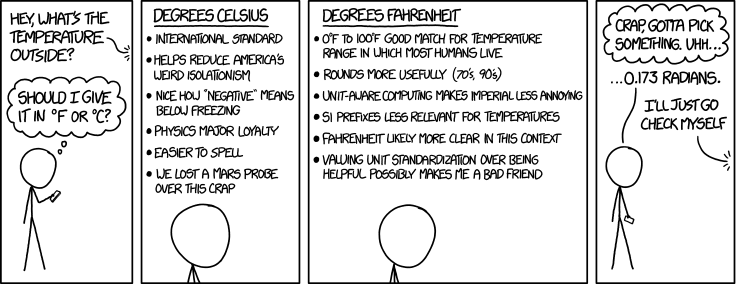
\includegraphics[width=0.75\textwidth]{degrees}
\end{center}
\end{figure}

\end{document}
